\chapter{Class F Amplifier ADS Simulations, Comparisons to Specs}

The initial goal of the class F amplifier design was to try and control up the fifth harmonic which would ideally allow 90.5\% drain efficiency and to have a center frequency of 5 GHz. After looking through the past amplifier competitions and looking at various RF transistor manufacturers, the Wolfspeed CGHV1F006S GaN HEMT transistor was chosen. This model was chosen over others to the relatively new release of the transistor, the high operating frequency of the transistor (18 GHz), and the fact that the transistor came in a QFP package versus a semiconductor die. The majority of past winners of the amplifier competition used Cree (now Wolfspeed) transistors and Wolfspeed provides a transistor level models for simulations to help design amplifiers. The design goals are in Table \ref{table:design_goal}, the initial goals were relatively aggressive in trying to push the PAE and center frequency for the highest figure of merit. After simulating, fabricating, and testing multiple versions the design goals were set to a more conservative value. This chapter discusses the simulations results of the final version of the amplifier. The initial design would have had a figure of merit of 120 which would be 10 points higher than the previous highest score in the competition. The final amplifier on the other hand would have a figure of merit of 92 which is still competitive with the past years submissions.

The initial design was pushing the limits of the specification by attempting to achieve the minimum output power with the highest allowed input power. This was risky because designing for the minimum gain allows for little margin for non-ideal factors that couldn't be taken into account of the simulation. The first amplifier that was fabricated had a simulated gain of 12 with a PAE of 80.1\% at an input power of 24 dBm. The amplifier initially had a short from the drain and had to be reheated with the a heatgun multiple times to fix the short. Once the amplifier was working the measured gain was only 10 dB so even at the maximum allowed input power of 24 dBm, it would not be able to deliver 36 dBm of power. For the final version of the amplifier, the design margins were increased substantially to compensate for fabrication issues and to ensure a working amplifier would be built even if the score was lower.

%REWORK

\begin{table}
    \centering
    \caption{Design Goals of Amplifier}
    \label{table:design_goal}
    \begin{tabular}{|l|l|l|}
      \hline
      % after \\: \hline or \cline{col1-col2} \cline{col3-col4} ...
      {Parameter}                      & {Initial Goal}     & {Final Goal} \\ \hline
      {Center Frequency, GHz}          & 5                  & 3 \\ \hline
      {PAE at Input Power, \%}         & 80                 & 70 \\ \hline
      {Output Power, dBm}              & {\textgreater 36}  & {\textgreater 36} \\ \hline
      {Input Power, dBm}               & 24                 & 15 \\ \hline
      {Input and Output VSWR}          & {\textless 2}      & {\textless 2} \\ \hline
    \end{tabular}
\end{table}

\section{DC Bias Point}
The simulation of the various parts of the class F amplifier was done using Keysight ADS 2016. The first step in the simulation process was determining the optimal DC bias. Using the provided transistor model from Wolfspeed, various drain and gate voltages were simulated to predict the drain current and transducer gain of the transistor using the circuit seen in Figure \ref{fig:bias_ckt}. The bias for the class F amplifier should be in the "deep" AB region so the drain current resembles a half sinusoid shape but still allows for the negative third harmonic to be present. The drain current should be minimized in order to maximize the PAE of the amplifier. The competition rule states the amplifier should have a minimum of 36 dBm output power at a maximum of 24 dBm input power resulting in a minimum gain of 12 dBm. For the final amplifier, the target gain was 21 dB at input power of 15 dBm so there would be a margin for various effects that wouldn't be able to be taken into account in the simulation like the fabrication process. So even if the gain was lower than 21 dB, at higher input power the amplifier would still be able to output at least the 36 dBm required.

\begin{table}
    \centering
    \caption{Maximum Operating Parameters of CGHV1F006S Transistor}
    \label{table:trans_param}
    \begin{tabular}{|l|l|}
      \hline
      % after \\: \hline or \cline{col1-col2} \cline{col3-col4} ...
      {Parameter} & {Rating}\\ \hline
      {Maximum Drain-Source Voltage, V} & 100 \\ \hline
      {Maximum Drain-Source Current, A} & 0.95\\ \hline
      {Maximum Gate-Source Voltage, V}  & -10,+2 \\ \hline
      {Maximum Gate-Source Current, mA} & 1.2 \\ \hline
    \end{tabular}
\end{table}

%Maybe include the recommended values?

The transistor maximum operating ratings can be seen in Table \ref{table:trans_param}. A starting point to select the gate voltage is to choose a value so the drain current is 10\% of the maximum current so the conduction cycle is close to $\pi$. The final version of the amplifier had a gate source voltage of -2.4 V which in Figure \ref{fig:ids_versus_vds} is in the "deep AB" region of the device and draws only 80 mA of quiescent current compared to the maximum drain current of 0.95 A. The drain-source voltage was chosen to be 40 V because it's the recommended operating voltage from the datasheet for the transistor. After the gate voltage was selected, the stability factor ($k$) and the stability measurement ($\Delta$) were then simulated to see what the stability of the amplifier is near the center frequency seen in Figures \ref{fig:stab_fact} and \ref{fig:stab_meas} respectively. For an amplifier to be unconditionally stable, $k$ must be greater than one and $\Delta$ be positive, and because $k$ is less than one the amplifier has potentially unstable regions. The stability regions of the load and source plane were then simulated to determine a starting point for the load and source pulls. The results of the load and source stability regions can be seen in Figures \ref{fig:load_stab} and \ref{fig:source_stab}. The region of stability for both stability circles is outside the circle.

%cite needed for stability factor stuff

\begin{figure}
  \centering
  % Requires \usepackage{graphicx}
  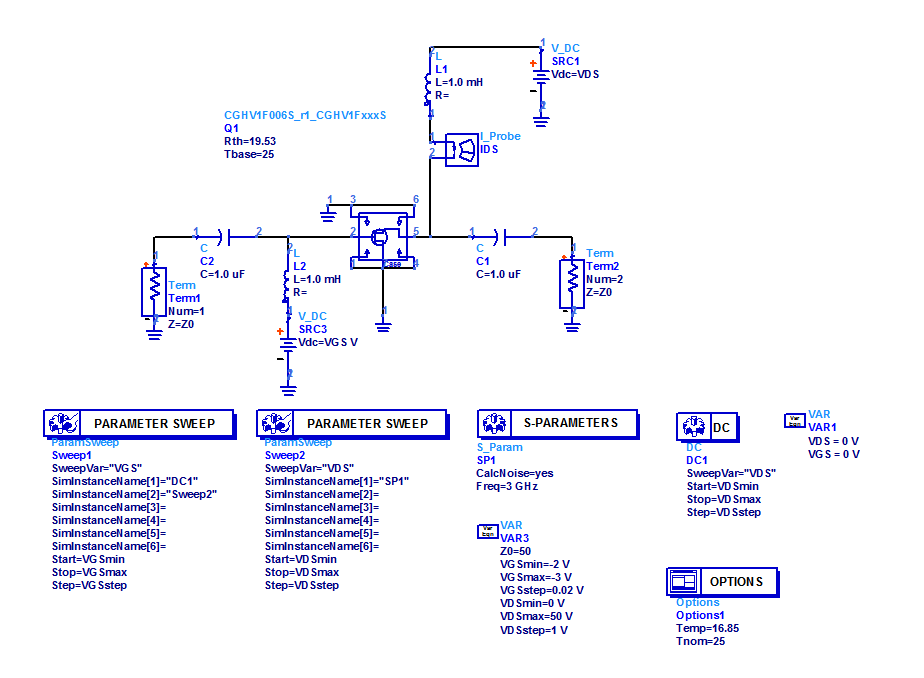
\includegraphics[width=6in,height=6in,keepaspectratio]{figures/simulation/bias_ckt}\\
  \caption{Bias Circuit Setup}
  \label{fig:bias_ckt}
\end{figure}

%Plot of Ids vs Vds and maximum transducer gain
\begin{figure}
  \centering
  % Requires \usepackage{graphicx}
  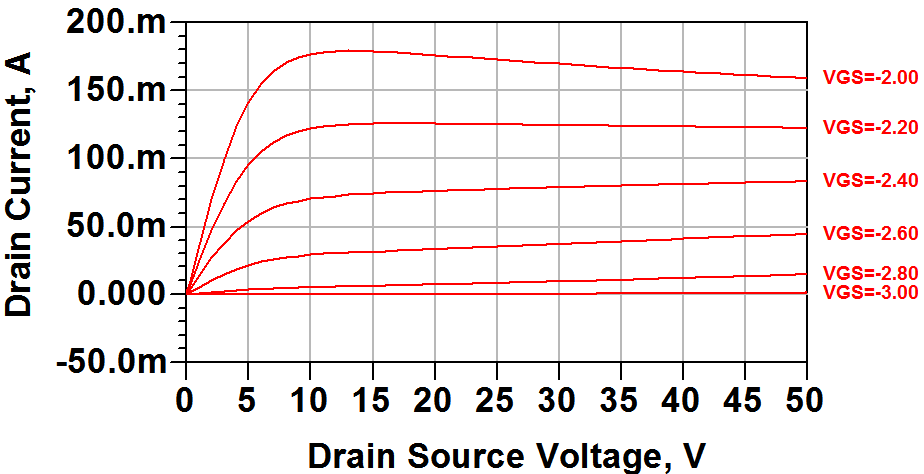
\includegraphics[width=5in,height=5in,keepaspectratio]{figures/simulation/ids_versus_vds}\\
  \caption{Drain Current versus Drain Voltage for Various Gate Voltages}
  \label{fig:ids_versus_vds}
\end{figure}

\begin{figure}
  \centering
  % Requires \usepackage{graphicx}
  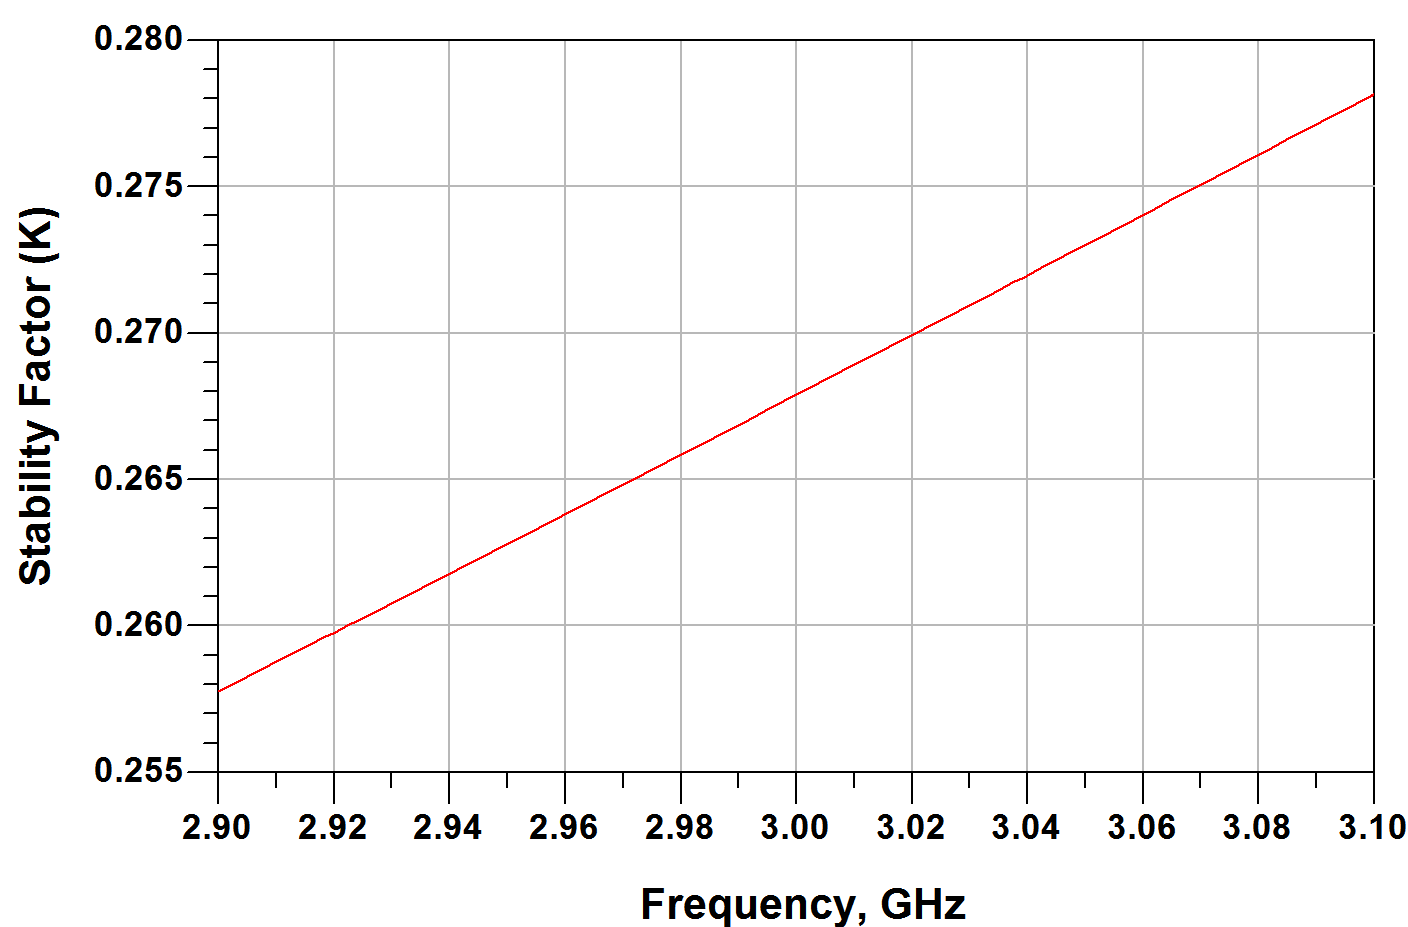
\includegraphics[width=5in,height=5in,keepaspectratio]{figures/simulation/stab_fact}\\
  \caption{Stability Factor ($k$) versus Frequency}
  \label{fig:stab_fact}

  \vspace*{\floatsep}

  \centering
  % Requires \usepackage{graphicx}
  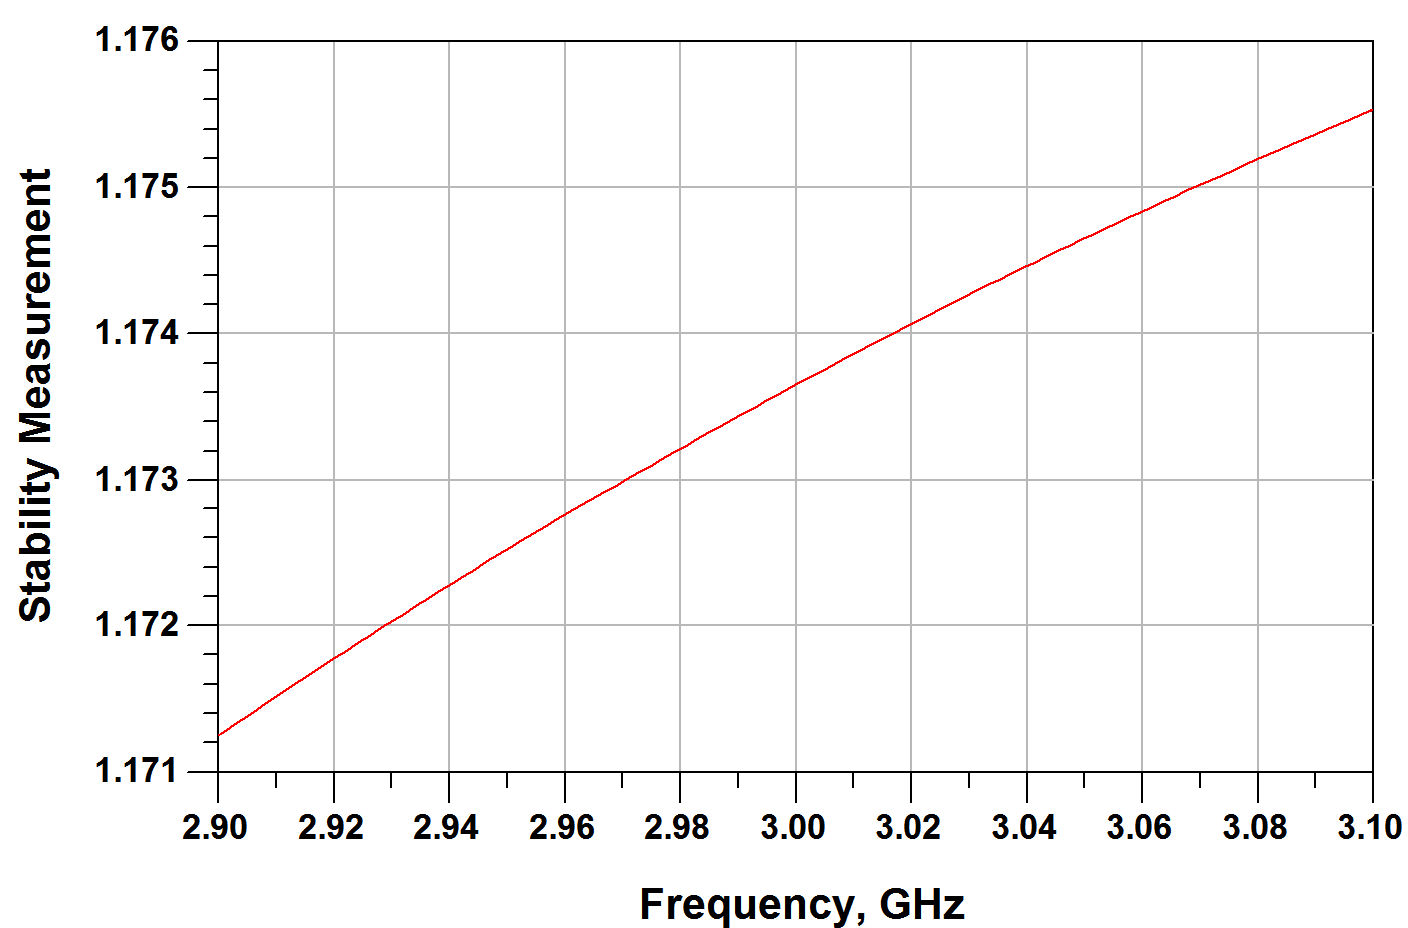
\includegraphics[width=5in,height=5in,keepaspectratio]{figures/simulation/stab_meas}\\
  \caption{Stability Measure ($\Delta$) versus Frequency}
  \label{fig:stab_meas}
\end{figure}

\begin{figure}
  \centering
  % Requires \usepackage{graphicx}
  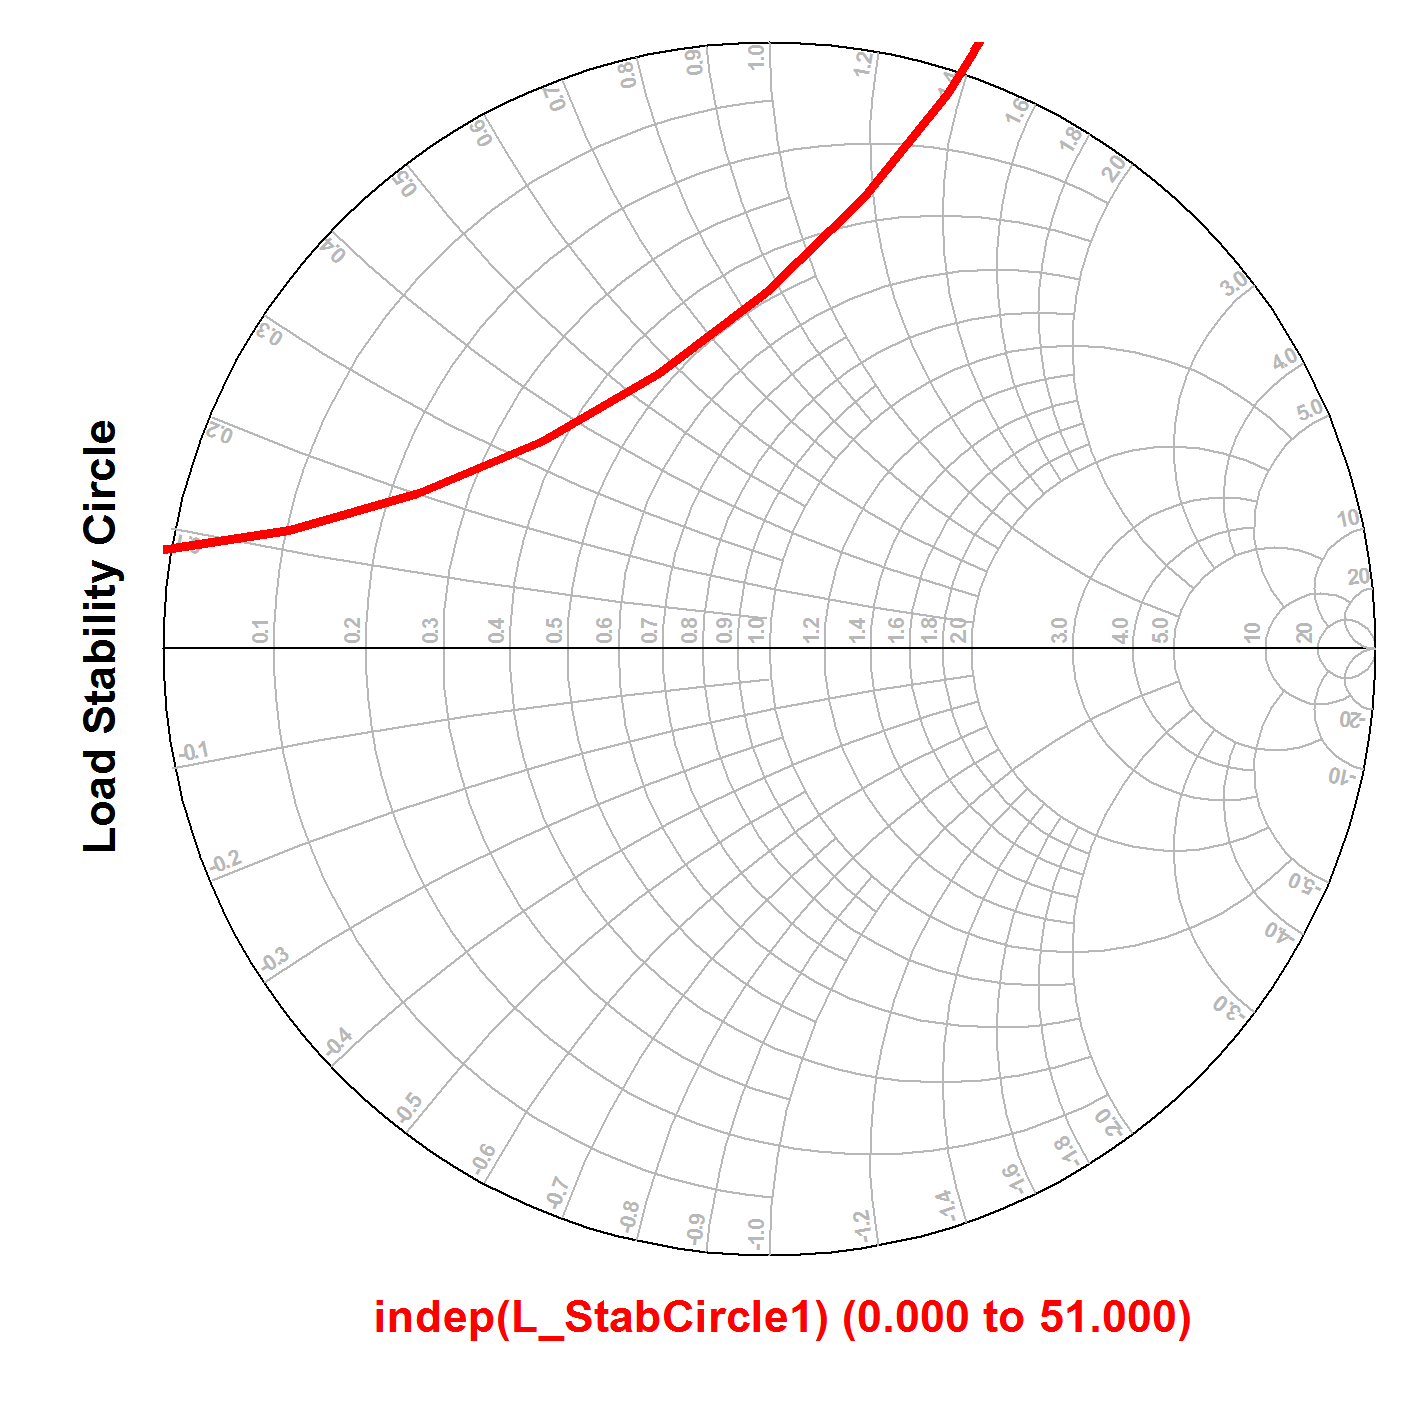
\includegraphics[width=4in,height=4in,keepaspectratio]{figures/simulation/load_stab}\\
  \caption{Load Stability Circle of Transistor. Stable Region Outside of Circle}
  \label{fig:load_stab}

  \vspace*{\floatsep}

  \centering
  % Requires \usepackage{graphicx}
  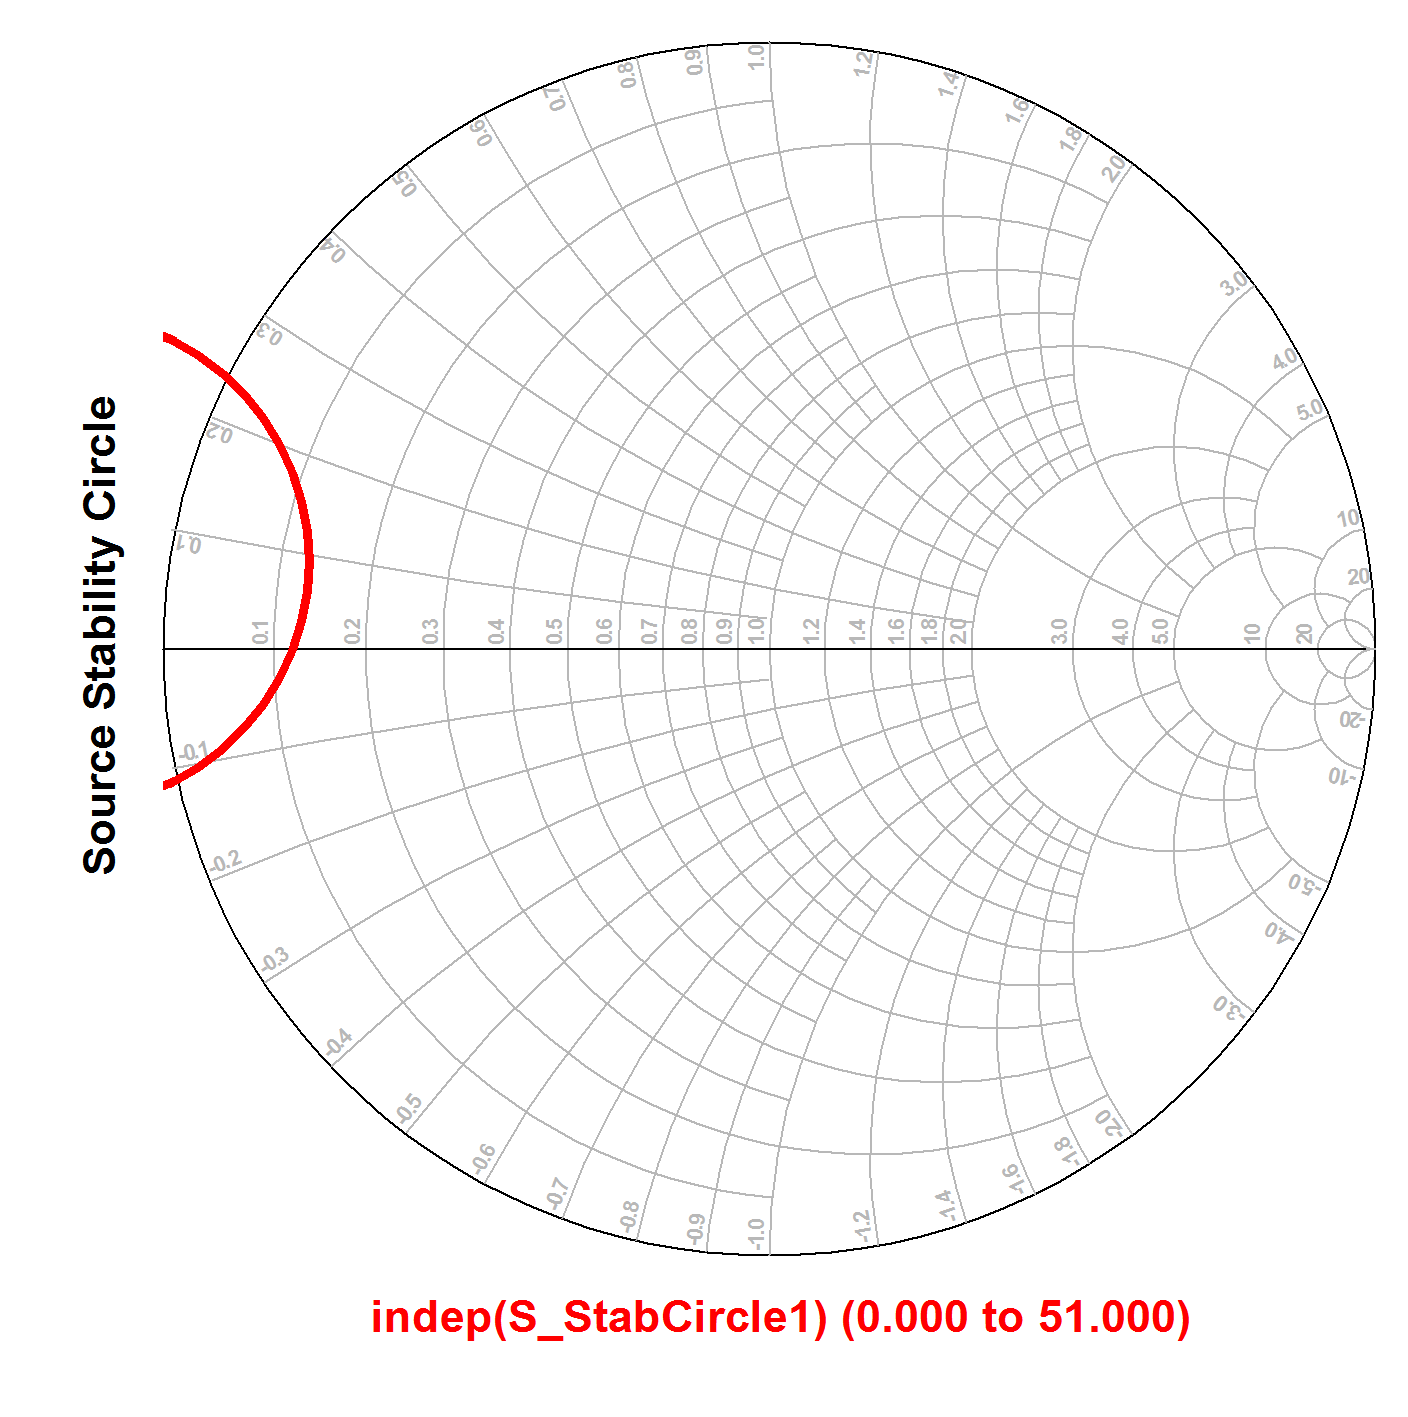
\includegraphics[width=4in,height=4in,keepaspectratio]{figures/simulation/source_stab}\\
  \caption{Source Stability Circle of Transistor. Stable Region Outside of Circle}
  \label{fig:source_stab}
\end{figure}

%Talk about simulation results

\section{Fundamental Load and Source Pull}

After determining the DC bias of the amplifier, fundamental load and source pulls are done to determine the optimal load and source impedances for the transistor. Load pulls are done keeping the source impedance fixed and sweeping the load over a uniformly sampled space on the Smith Chart and measuring the transducer gain and PAE. Various gain and PAE contours can be produced by doing load pulls. The process starts with sampling the entire Smith Chart then load pulling again around the region with the highest efficiency contour to find the optimal load impedance. As a starting point the source impedance was set to a low impedance of 10$\Omega$ that was within the stable region on the source side. Source pulling is done after load pulling and follows a similar process by keeping the load impedance fixed then sweeping the source impedance for the highest efficiency while still having the target gain. The load and source pulls are done at the fundamental frequency at an input power of 15 dBm to provide an additional margin in the design. In practice the amplifier the amplifier will require a higher input power to achieve the simulation results due to losses that could not be simulated in ADS. Also for the fundamental load and source pull, the source and load impedances for the higher harmonics are shorted.

For the sake of brevity only the final load and source pull results are shown but the general process will be described. The initial load pull results showing PAE and power delivered contours can be seen in Figure \ref{fig:smith_fund_load} and \ref{fig:xy_fund_load}. The highest power delivered is only 35.45 dBm at a drain efficiency of 35\% while the highest PAE 40\% results in a power delivered of 35.2 dBm. The PAE should be less than 50\% because an amplifier with only the fundamental present is a class A amplifier with a maximum efficiency of 50\%. As more harmonics are properly added the power delivered and PAE should increase. The final fundamental load impedance selected from the simulation results was 14.3+j54 $\Omega$.

%REWORK next section talks about the final results

%Plots of load pull with efficiency and gain contours
\begin{figure}
  \centering
  % Requires \usepackage{graphicx}
  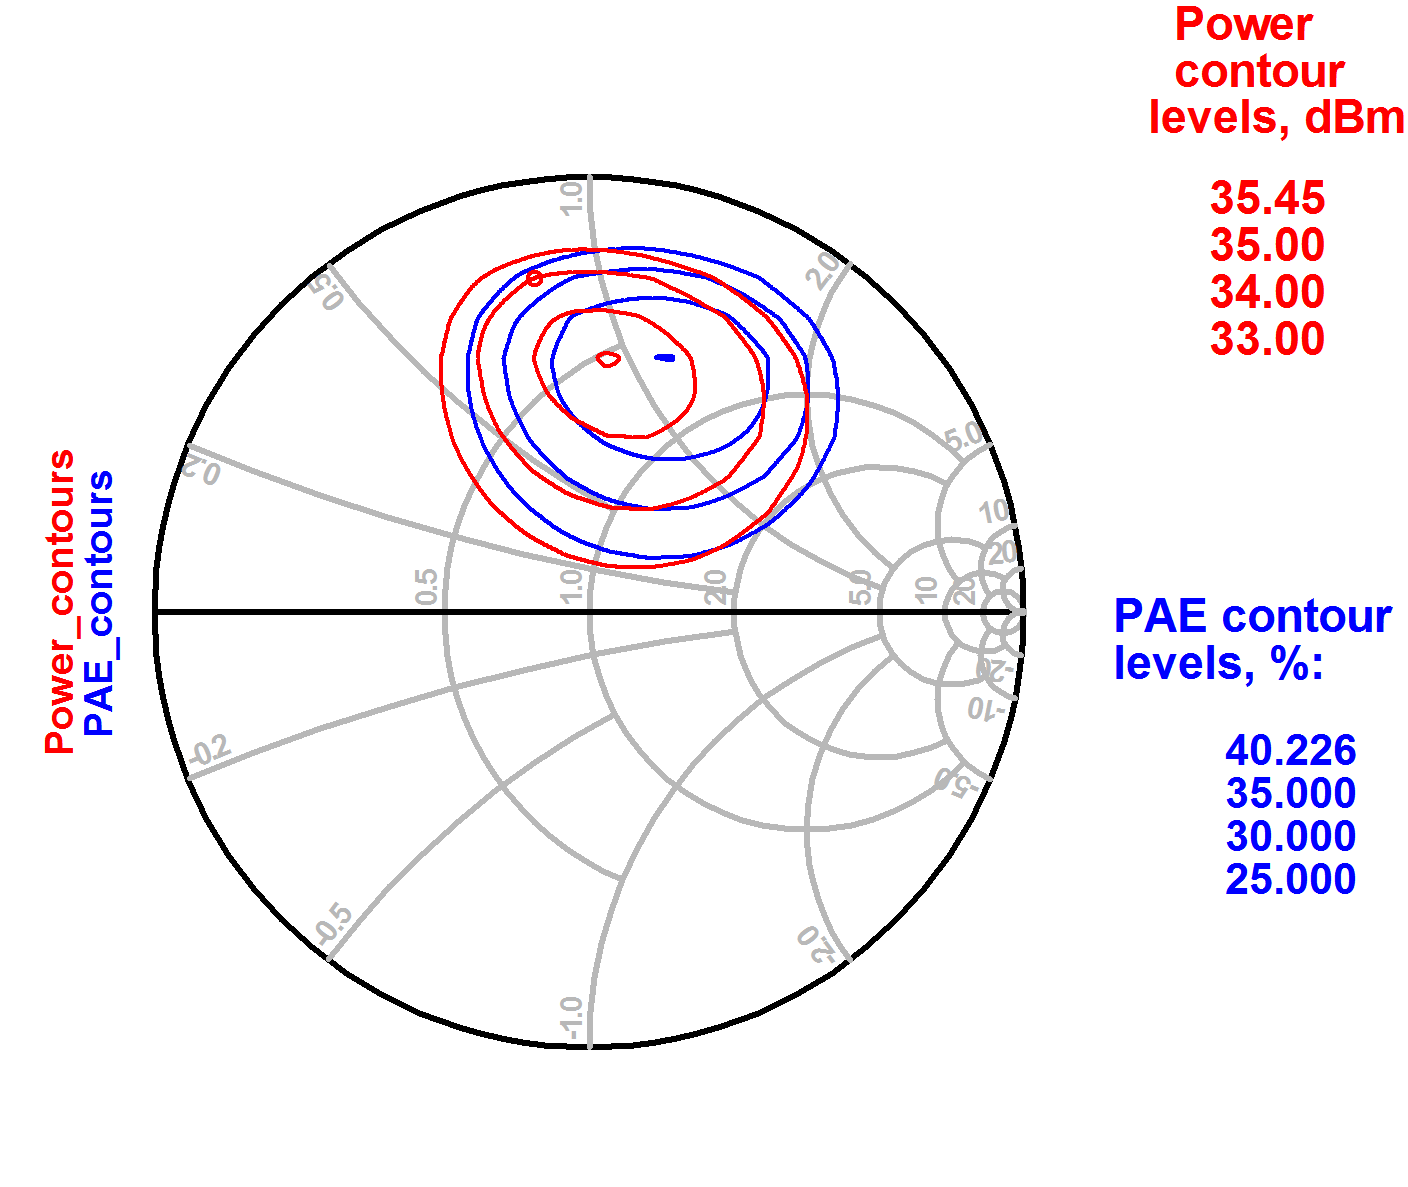
\includegraphics[width=4in,height=4in,keepaspectratio]{figures/simulation/pae_pout_smith_cont_fund}\\
  \caption{Initial Smith Chart Load Pull Simulation Results at 3 GHz}
  \label{fig:smith_fund_load}

  \vspace*{\floatsep}

  \centering
  % Requires \usepackage{graphicx}
  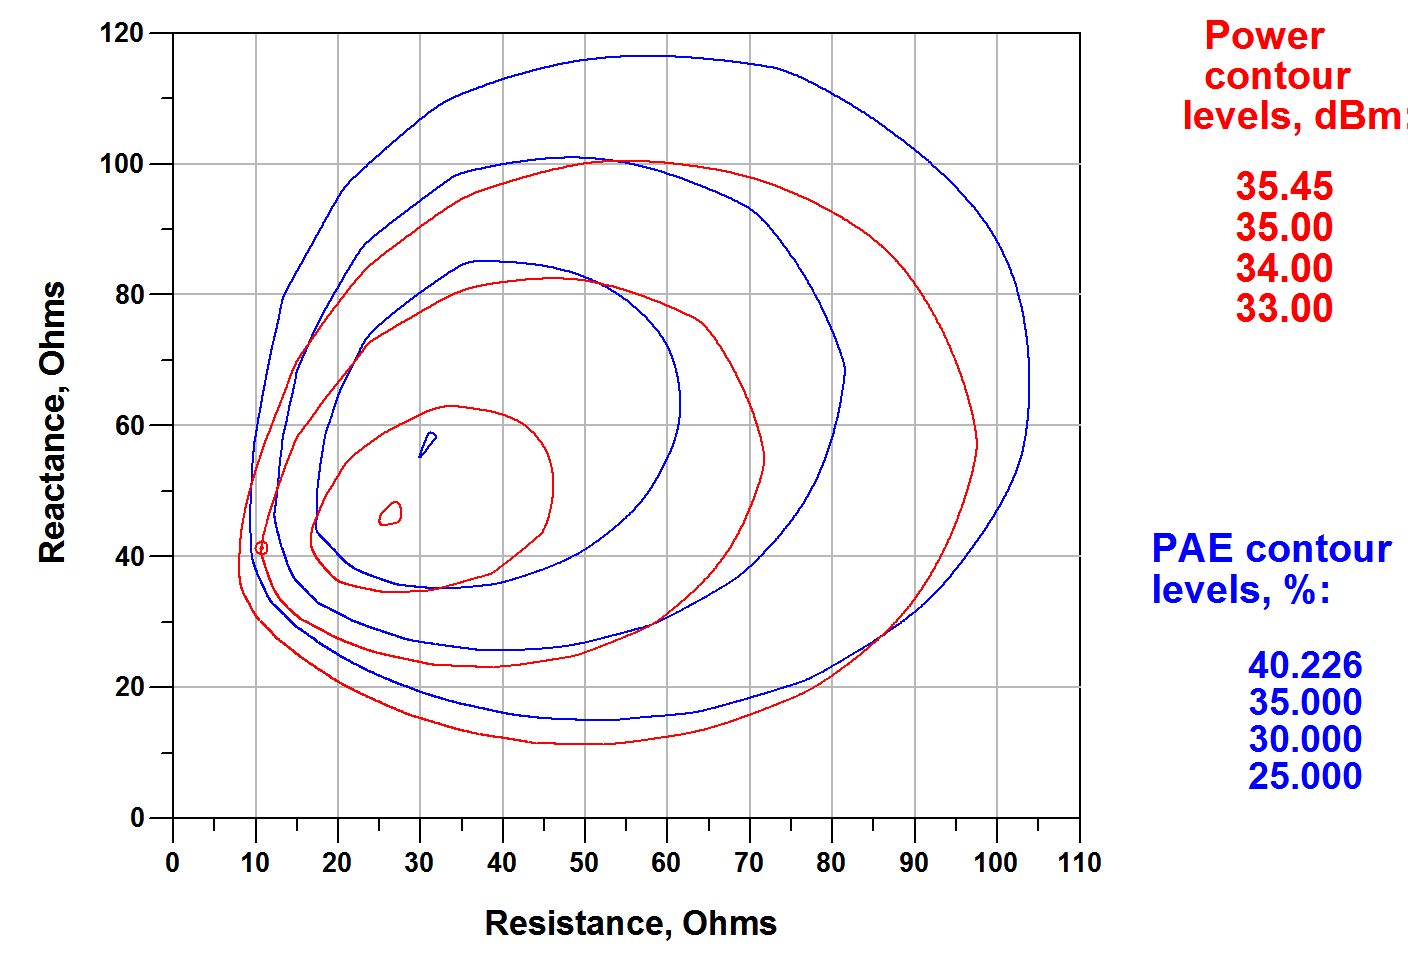
\includegraphics[width=4in,height=4in,keepaspectratio]{figures/simulation/pae_pout_res_cont_fund}\\
  \caption{Initial Reactance vs Resistance Load Pull Simulation Results at 3 GHz}
  \label{fig:xy_fund_load}
\end{figure}

%Plots of source pull with same as above

The next step is the source pull done with the load set to the impedance found in the load pull. The results of the initial source pull can be seen in Figures \ref{fig:smith_fund_source} and \ref{fig:xy_fund_source}. The maximum PAE and power delivered has dropped but this isn't unexpected. The pulling process is iterative and if another load pull was done using a new source impedance, the PAE and power delivered increase from the first load pull. Multiple iterations are required to fine tune the parameters because they are dependent on one another. A fundamental source impedance of 3+j3 $\Omega$ was chosen for the final amplifier configuration as a compromise between high PAE while still delivering over 36 dBm of power.

\begin{figure}
  \centering
  % Requires \usepackage{graphicx}
  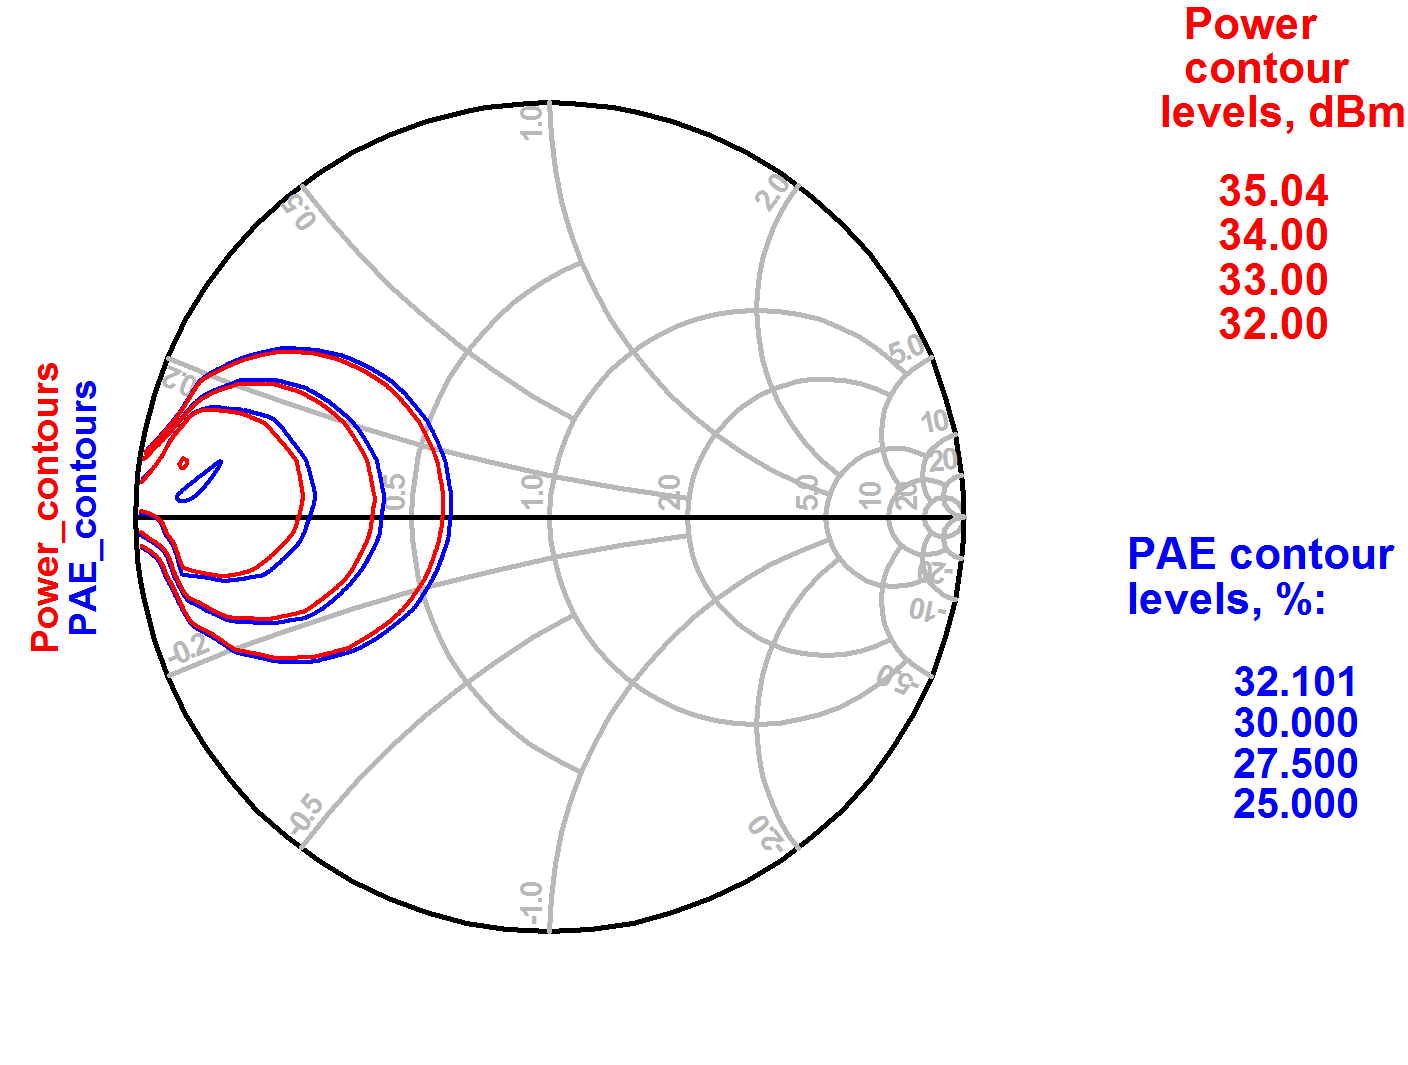
\includegraphics[width=4in,height=4in,keepaspectratio]{figures/simulation/smith_fund_source}\\
  \caption{Initial Smith Chart Source Pull Simulation Results at 3 GHz}
  \label{fig:smith_fund_source}

  \vspace*{\floatsep}

  \centering
  % Requires \usepackage{graphicx}
  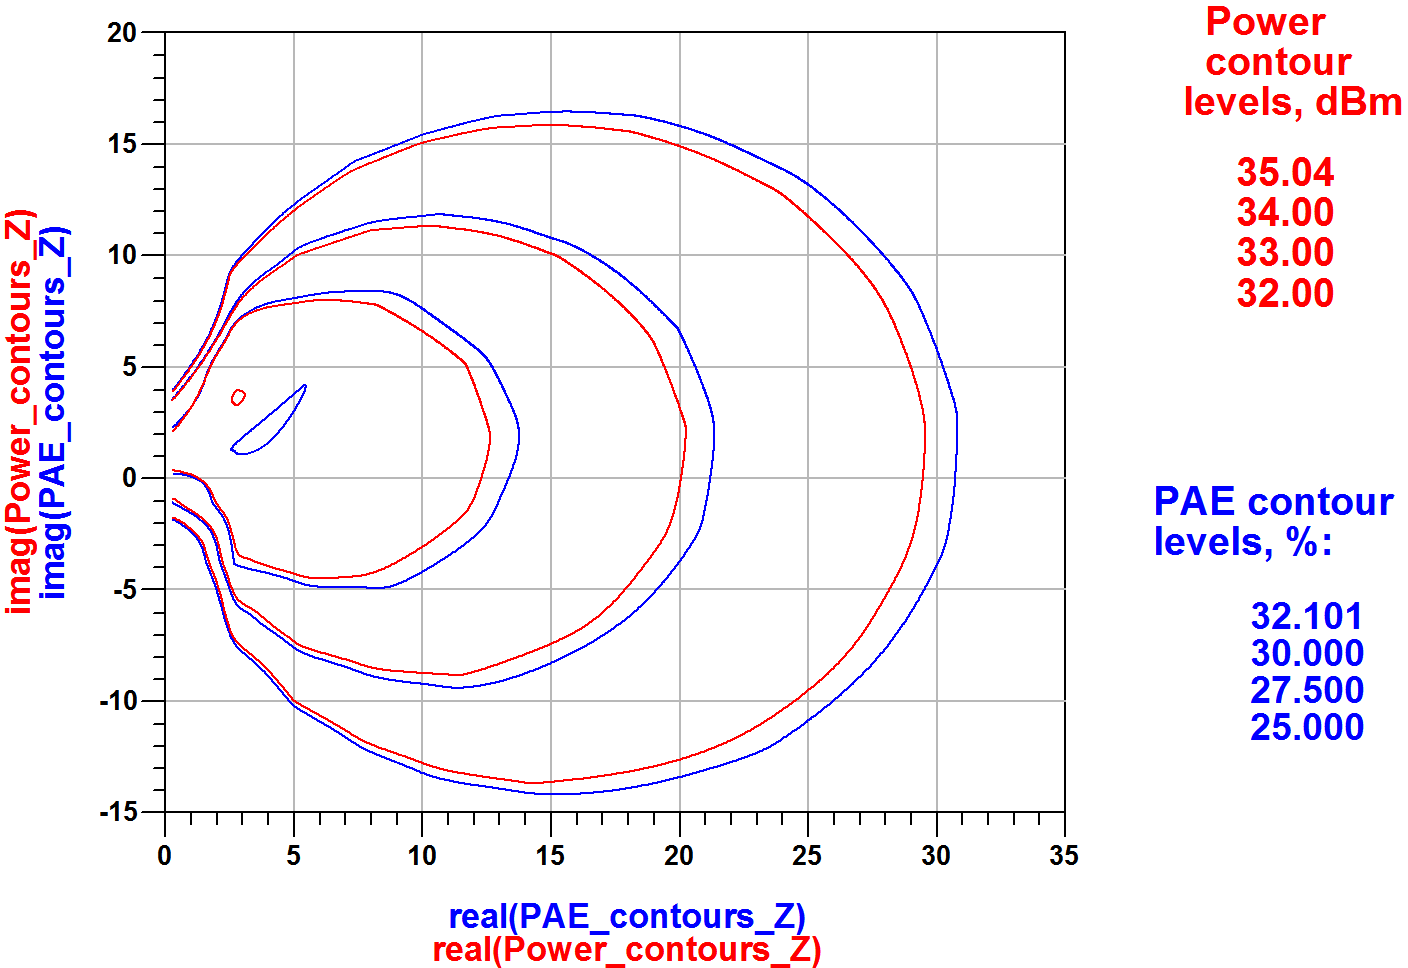
\includegraphics[width=4in,height=4in,keepaspectratio]{figures/simulation/res_fund_source}\\
  \caption{Initial Reactance vs Resistance Source Pull Simulation Results at 3 GHz}
  \label{fig:xy_fund_source}
\end{figure}

%Talk about simulation results

\section{Harmonic Load and Source Pulls}

The load and source pulls are done at the fundamental frequency while the harmonic pulls are done at the higher harmonics. The process starts with the second harmonic load pull with the fundamental load and source impedances set to the values determined in the previous section. The source impedance at the second harmonic and all the higher harmonic impedances are set to 0 $\Omega$. After determining the optimal load for maximum PAE while still delivering enough output power, a source pull is done at the second harmonic with the optimal load. This process is then repeated for at the third harmonic. After all of the load and source pulls, one last load pull is done at the fundamental to confirm an the increase of PAE and power delivered at the fundamental frequency. The final fundamental load pull can be seen in Figure \ref{fig:sc_fund_final_load} and \ref{fig:res_cont_fund_load_final}. At the highest power delivered of 38.9 dBm the PAE is 69\% while at the highest PAE of 79\% the output delivered is 36.9 dBm.

A table of the load and source impedances used for the final amplifier configuration can be seen in Table \ref{table:harmonic_impedance}. The final amplifier had an output power of 37 dBm with 22 dB of gain and a PAE of 79.25\% resulting in a figure of merit of 104. While the figure of merit is not the highest compared to the past winners, it is still competitive. The drain efficiency of the final amplifier is 79.2\% which is close to the theoretical maximum of 81.7\%. The simulated harmonic pulls are used to determine the maximum theoretical performance that can be extracted from the transistor. The PAE and output power of the amplifier with physical transmission lines will be less than the ideal case.

\begin{table}
    \centering
    \caption{Final Harmonic Impedances for Amplifier}
    \label{table:harmonic_impedance}
    \begin{tabular}{|l|l|l|} \hline
    % after \\: \hline or \cline{col1-col2} \cline{col3-col4} ...
    {Frequency, GHz} & {Load Impedance, $\Omega$} & {Source Impedance, $\Omega$} \\ \hline
    {3} & {14.3+j54.0} & {3+j3} \\ \hline
    {6} & {1.4+j37.0} & {3-j55} \\ \hline
    {9} & {0.3+j13.4} & {0.5-j2.6} \\ \hline
    \end{tabular}
\end{table}

\begin{figure}
  \centering
  % Requires \usepackage{graphicx}
  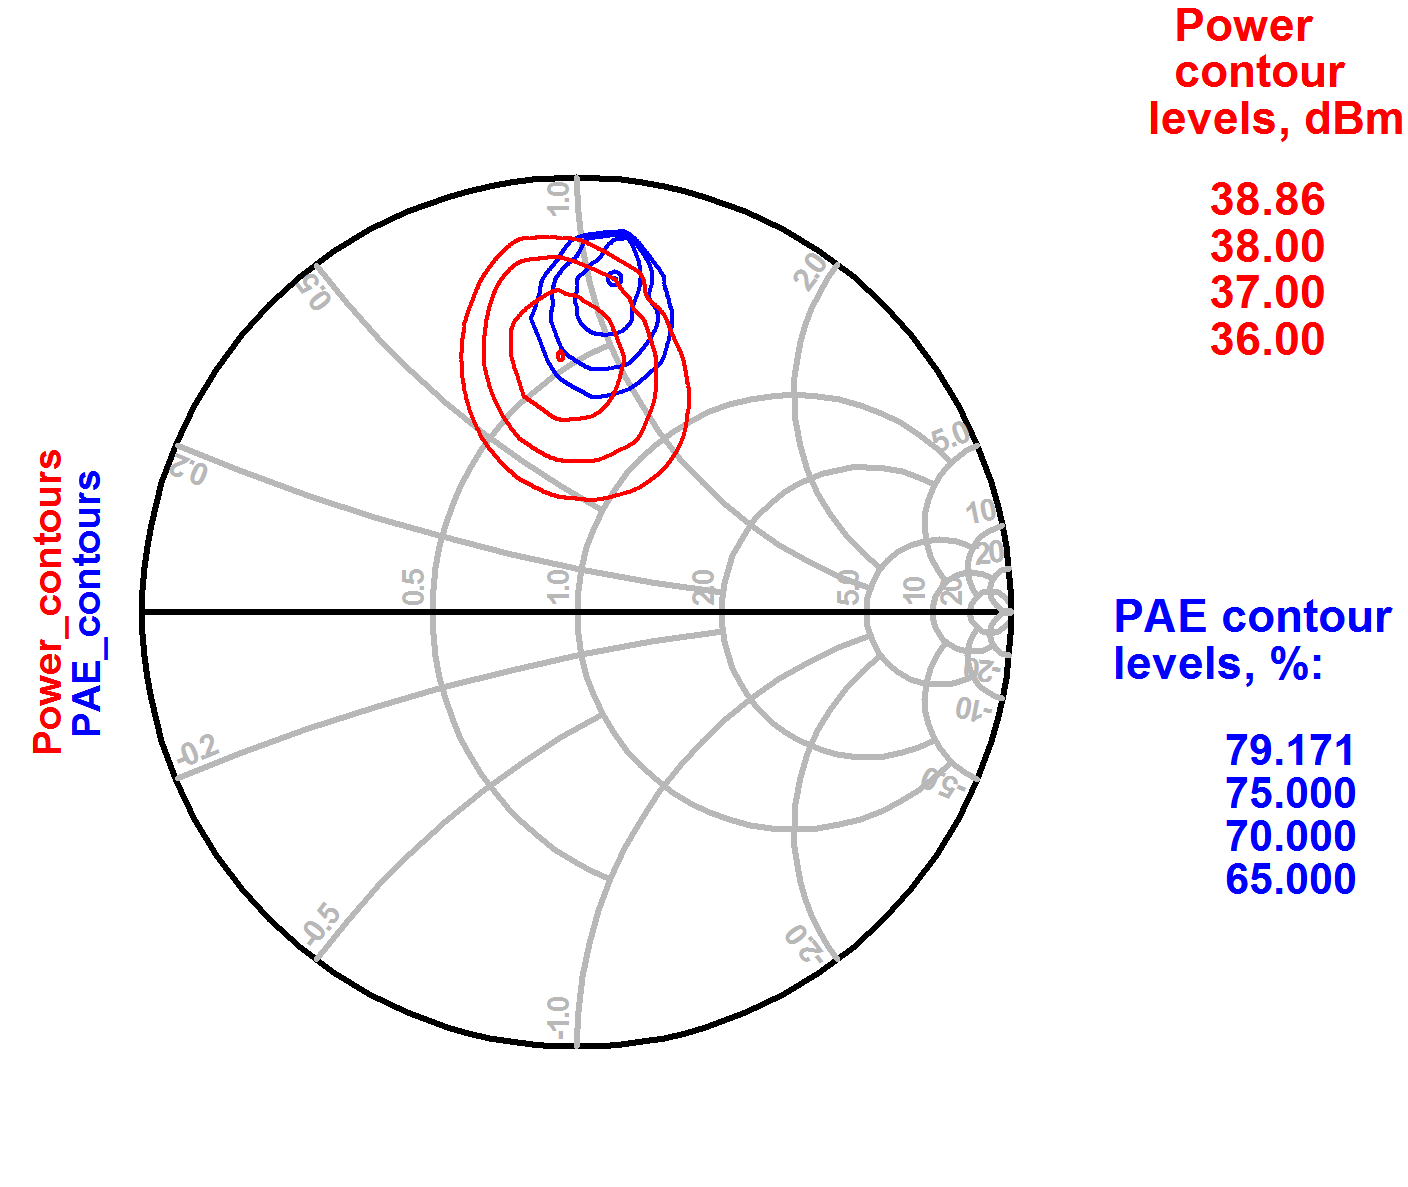
\includegraphics[width=4in,height=4in,keepaspectratio]{figures/simulation/sc_fund_final_load}\\
  \caption{Final Fundamental Smith Chart Load Pull}
  \label{fig:sc_fund_final_load}

  \vspace*{\floatsep}

  \centering
  % Requires \usepackage{graphicx}
  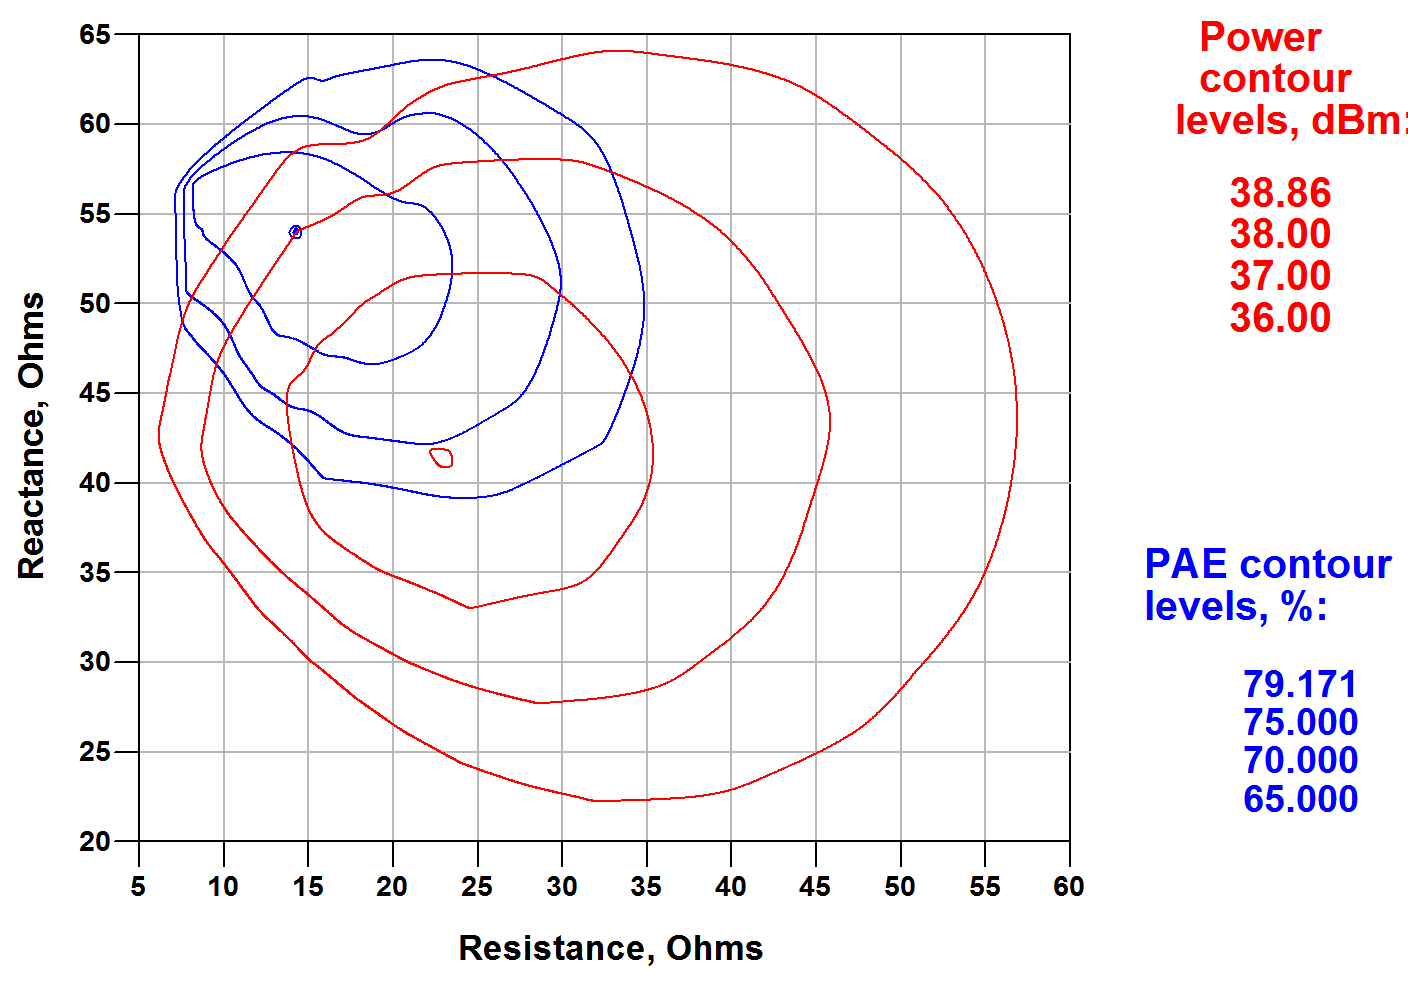
\includegraphics[width=4in,height=4in,keepaspectratio]{figures/simulation/res_cont_fund_load_final}\\
  \caption{Final Fundamental Reactance vs Resistance Load Pull}
  \label{fig:res_cont_fund_load_final}
\end{figure}

%%The harmonic phase pull is done at the lowest harmonic from load to source then to the highest harmonic. The harmonic phase pull is done at the input and output because it's been shown experimentally that harmonic matching networks at the input can also increase the drain efficiency INSERT REFERENCE HERE. The harmonic phase pull can measure gain and efficiency contours just like the load and source pulls. The end result of all the various pull simulations is the ideal gain and efficiency of the amplifier in class F operation if the harmonics are ideally terminated. The process of determining a DC bias, fundamental load and source pull, and harmonic phase pulls is repeated until the requirements are met. Table X shows the iteration steps and amplifier performance. Initially the goal was to control up to the fifth harmonic to hopefully increase the efficiency near the theoretical value of 90.5\% CHECK THIS VALUE. But this the transistor used there weren't any sufficient gains from controlling up to the third harmonic versus controlling up to the fifth harmonic so it was decided only up to the third harmonic will be controlled.

%Harmonic phase pull with contours

%Final simulated parameters of transistor

\section{Harmonic Matching Network}

The harmonic matching network is the key in keeping the proper harmonics at the drain. It is composed of a matching network and a wave shaping network that is on the load and source side of the transistor. The wave shaping network consists of a series section that is a quarter wavelength long with an eight wavelength open shunt stub. An additional series element is added that is used for tuning that goes to a two more stubs that used for the second harmonic and bias circuitry seen in Figure \ref{fig:matching_network_woo}. Most class F wave shaping network follow a similar pattern of various fractional wavelength sections so the harmonics at the drain are properly terminated. The downside of these networks is the relatively large electrical lengths due to the presence of a quarter wavelength sections in nearly all such networks. This design explores if coupling the open circuit shunt stubs in the wave shaping network can decrease the electrical size of the class F amplifier. Two versions of the amplifier were simulated, one that uses coupled microstrip lines and one without to compare the overall electrical size of the amplifier. After the wave shaping network comes the matching network so the amplifier is matched as close as possible to 50$\Omega$. This amplifier used a shunt stub and a series transmission line for the matching network on the load and source side. The matching networks were designed to match to 50 $\Omega$.

%Insert figure of matching network and wave shaping network
\begin{figure}
  \centering
  % Requires \usepackage{graphicx}
  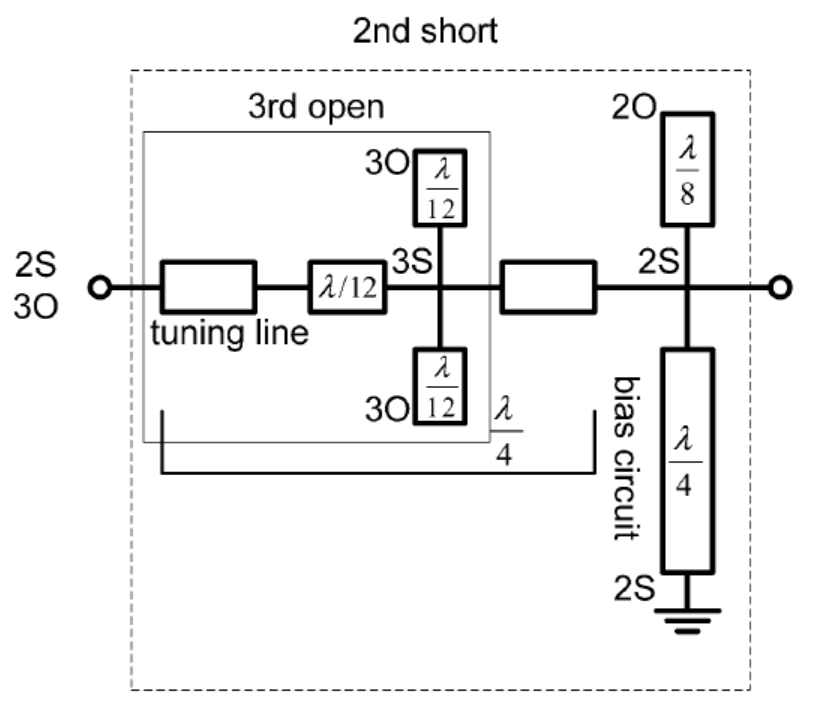
\includegraphics[width=4in,height=4in,keepaspectratio]{figures/simulation/matching_network_woo}\\
  \caption{Matching Network for Amplifier} %cite woo
  \label{fig:matching_network_woo}
\end{figure}

\section{Simulated Amplifier}
After simulating the maximum theoretical performance of the class F amplifier, the amplifier was simulated using the harmonic matching network discussed previously. Microstrip was chosen as the transmission line to be used for the harmonic matching network because the milling machine that was used to fabricate the boards could only remove the top layer of a copper clad board. Coplanar waveguide was also considered but not chosen because it would greatly reduce the bit life of the fine milling parts. The transmission lines were simulated using Rogers RO3035 with a dielectric constant of 3.5$\pm$0.05 with a thickness of 60 mil. R03035 was chosen after comparing various low loss laminates like Duroid from Rogers Corporation. This was partially due to the larger sample size that could be ordered so more amplifier boards could be fabricated. Also it has the lowest tangent loss and dielectric constant that allowed the transmission lines going to the transistor gate and drain to be narrow enough make contact without shorting to the ground pins on the package. Duroid was used for the first version of the amplifier and complications arose due to the width of the microstrip line going in to the transistors drain and gate pins. Using high dielectric constant materials like RT/duroid 6010 with a dielectric constant of 10.2$\pm$0.25 resulted in dimensions to narrow to be fabricated on the milling machine. The board discussed in this section is the third revision. The previous two amplifiers malfunctioned with one acting as an oscillator and the other not working at all. This was most likely due to fabrication issues because of the leadless package of the transistor.

Two versions of the amplifier were simulated to compare the electrical length of the harmonic matching network with coupled stubs and without. The harmonic matching network in Figure \ref{fig:matching_network_woo} was used as the starting point in the design. The Linecalc tool in ADS used to calculate the quarter, eighth, and twelfth wavelength at the center frequency of 3 GHz on the R03035 laminate. One key element lacking from the fractional wavelength based harmonic matching network is any analysis of the impedances for the sections of the transmission lines. A majority of papers seem to fix the transmission line length and then leave the impedances of each line to be determined by an optimizer. The load and source side of the matching networks were initially optimized independently of each other. To optimize the load matching network, the source impedance was set to the fundamental value of 3+j3 $\Omega$ then the width of the microstrip lines were optimized for maximum PAE and an output power greater than 36 dBm at an RF input power of 15 dBm. The same process was done with the source matching network by fixing the load impedance to 14.3+j54.0 $\Omega$ and repeating the optimization. The overall goal for this was to try and approach the global optimum for the load and source matching networks separately and also minimize the number of variables the optimizer in ADS would have to tune. After tuning the load and source sides of the harmonic matching networks independently of one another, both sides were then connected to the transistor. Further optimization was applied to fine tune the performance of the amplifier.

This process was repeated with coupled and not coupled microstrip lines for the shunt stub parts of the harmonic matching network. The total series length of the microstrip lines used in the designs was used to compare the electrical size of the two amplifiers. The total series length of the non-coupled amplifier was 6484 mils while the coupled amplifier was 3735 mils which is a 57.6\% reduction in size. While this was only done at a single frequency, bias and matching network; coupling the stubs in the matching network is shown here to reduce the electrical size of the class F amplifier. The original plan for the thesis was to test if coupling the matching networks works for various types harmonic matching networks that use transmission lines. Unfortunately due to time constraints that arose trying to build a working amplifier only one matching network was tested.

The amplifier was simulated using the harmonic balance and large signal s-parameters tools of ADS. Harmonic balance allows for proper simulation of non-linear devices by taking in account harmonic distortion by assuming a Fourier series steady state solution exists for any given circuit. The harmonic balance simulation is done in the frequency domain and is done by exciting the circuit with multiple tones with a given power. Linear elements in a circuit can be solved in the frequency domain while non-linear elements are sampled in the time domain and then converted in the frequency domain. This allows for accurate simulation of large signal devices like power amplifiers were inter-modulation and harmonic distortion occurs. If the amplifier was simulated using small signal s-parameters the harmonic generation at the drain of the transistor would not be taken into account because s-parameters uses a small signal model which assumes a non-linear device can be assumed to have linear properties at a specific bias. The large-signal s-parameter simulation uses the harmonic balance simulation results to produce s parameter results of a device.

The simulated drain current and voltage waveforms can be seen in Figure \ref{fig:ids_vds_wave} which show some partial overlap during switching. Although the waveforms aren't ideal, the amplifier still has high PAE and meets the minimum output power. Even during the off cycle of the drain current, there is still quiescent current flowing which dissipates significant power due to the high drain voltage. Figure \ref{fig:singletonesweep} shows the amplifier performance at 3 GHz from an input power of -30 dBm to 30 dBm. The amplifier is able to achieve an output power of 36 dBm at input powers greater than 11 dBm. The amplifier is able to achieve a peak PAE of 78\% at 19 dBm of input power resulting in a figure of merit score of 103. For the high PAE, the amplifier is operating beyond the 1 dB compression point which hints at the presence of intermodulation distortion. The simulated VSWR can be seen in Figure \ref{fig:amp_sim_vswr}, and load and source stability circles in Figures \ref{fig:amp_sim_load_stab} and \ref{fig:amp_sim_source_stab} which show the amplifier is stable at 50$\Omega$ at the center frequency.

%A two tone test was done at 3 GHz with two carriers 5 MHz apart.

%Talk about harmonic distortion of the amplifier. That's what the single tone IMD data represents.

%Table comparing the initial simulation specifications and the final simulation results
\begin{table}
    \centering
    \caption{Comparison of the Specification and Simulated Performance of Amplifier}
    \label{table:sim_spec_compare}
    \begin{tabular}{|l|l|l|}
      \hline
      % after \\: \hline or \cline{col1-col2} \cline{col3-col4} ...
      {Parameter}                      & {Specification }   & {Simulation} \\ \hline
      {Center Frequency, GHz}          & 3                  & 3 \\ \hline
      {Input Power for Max PAE, dBm}    & 15                 & 19 \\ \hline
      {Output Power for Max PAE, dBm}  & {\textgreater 36}  & {37.5} \\ \hline
      {Maximum PAE, \%}                & 70                 & 78 \\ \hline
      {Input and Output VSWR}          & {\textless 2}      & {\textless 2} \\ \hline
    \end{tabular}
\end{table}

%Drain current and voltage waveforms
\begin{figure}
  \centering
  % Requires \usepackage{graphicx}
  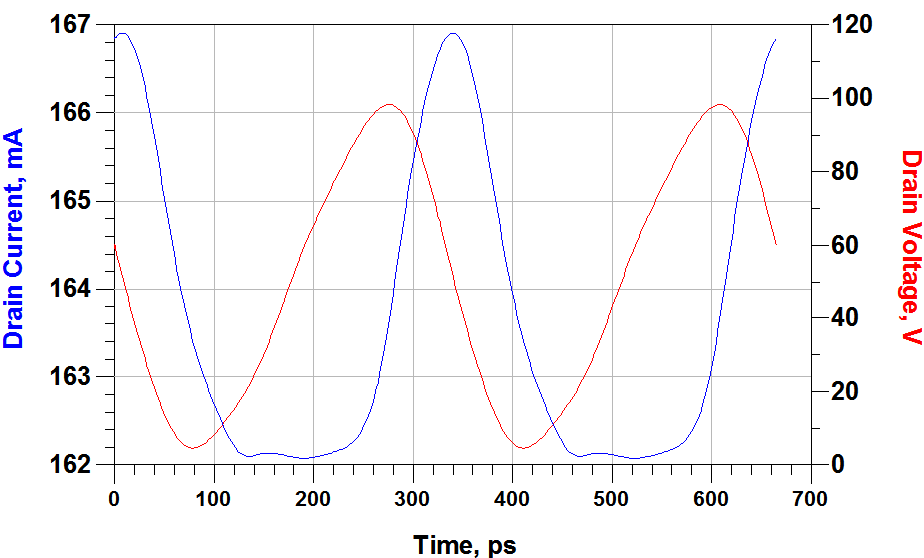
\includegraphics[width=5in,height=5in,keepaspectratio]{figures/amp_sim/ids_vds_wave}\\
  \caption{Simulated Drain Current and Voltage Versus Time}
  \label{fig:ids_vds_wave}

  \vspace*{\floatsep}

  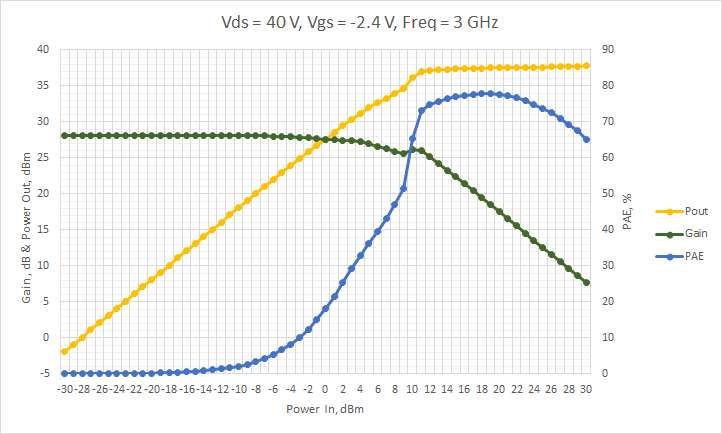
\includegraphics[width=5in,height=5in,keepaspectratio]{figures/amp_sim/singletonesweep}\\
  \caption{Gain, PAE, and Output Power versus Input Power}
  \label{fig:singletonesweep}

\end{figure}


%Two tone test
\begin{figure}
  \centering
  % Requires \usepackage{graphicx}
  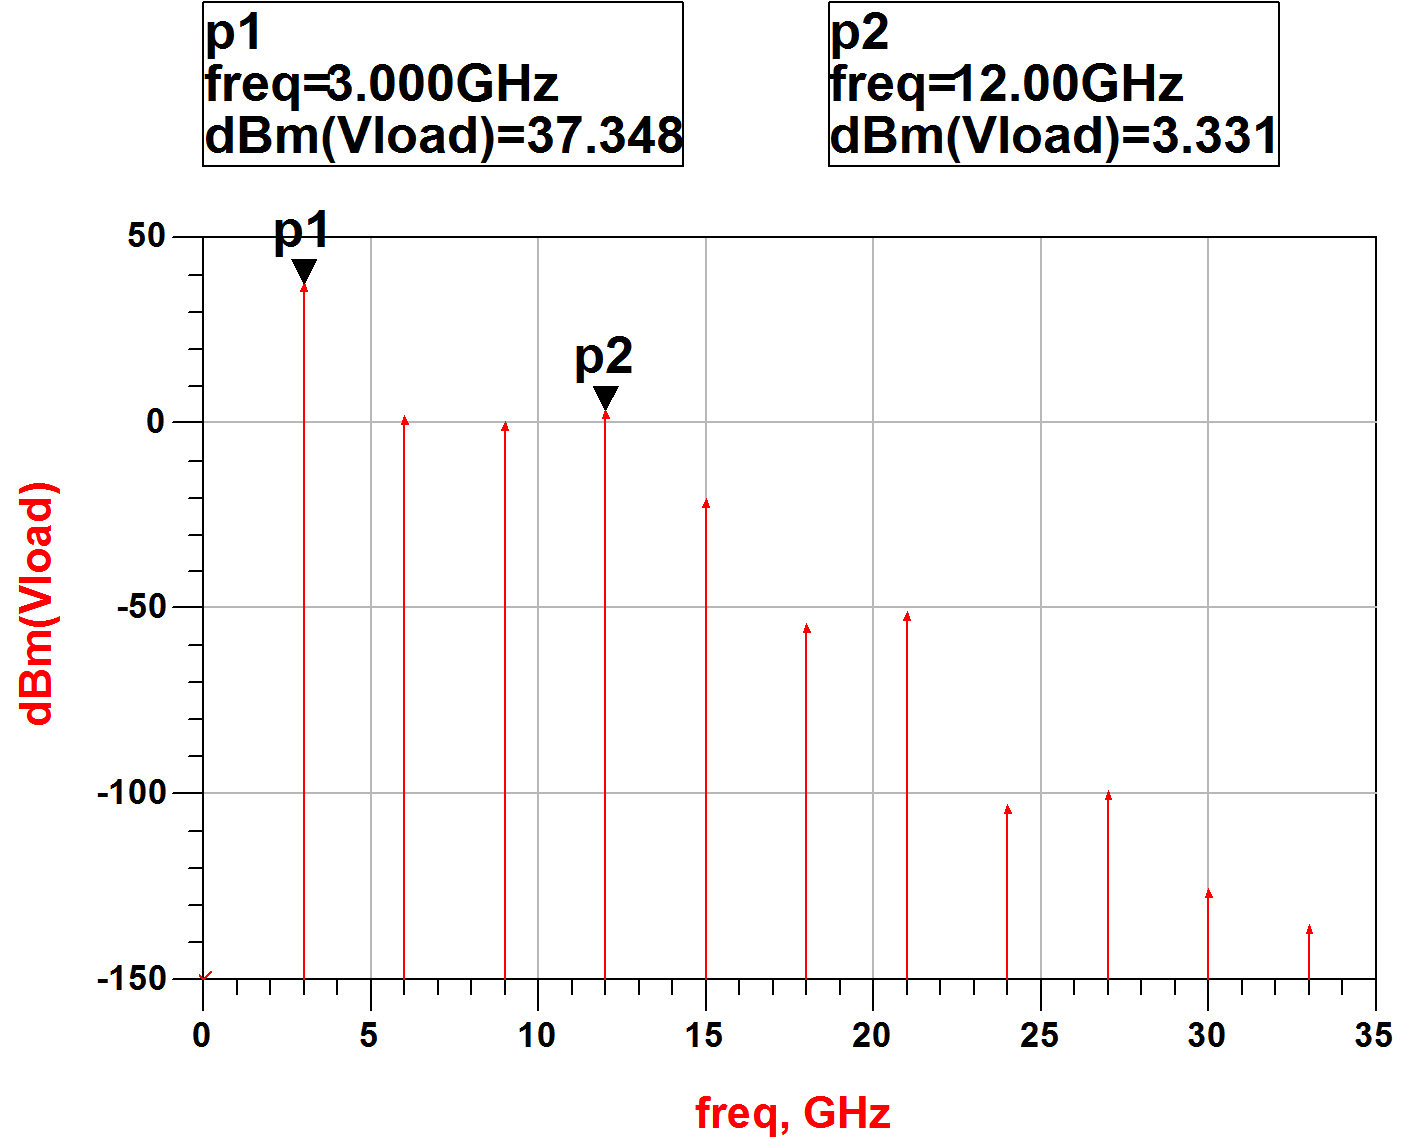
\includegraphics[width=5in,height=5in,keepaspectratio]{figures/amp_sim/IMD_singletone}\\
  \caption{Simulated Single Tone IMD}
  \label{fig:imd_single}

  \vspace*{\floatsep}

  \centering
  % Requires \usepackage{graphicx}
  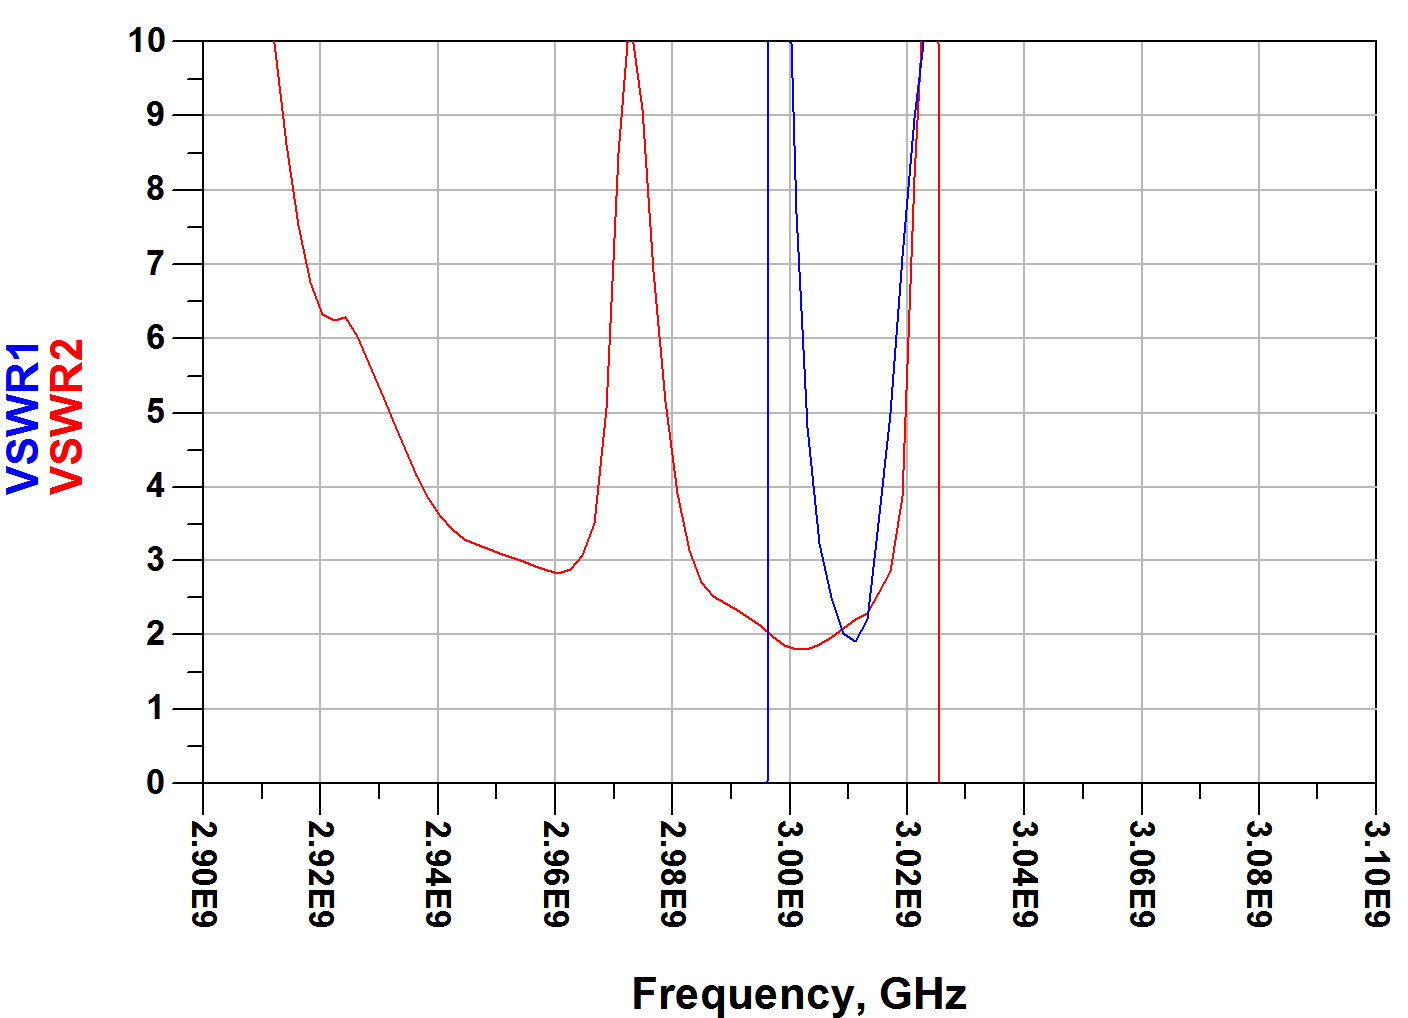
\includegraphics[width=5in,height=5in,keepaspectratio]{figures/amp_sim/vswr}\\
  \caption{Simulated Input (1) and Output (2) VSWR of Amplifier}
  \label{fig:amp_sim_vswr}

%    \centering
%  % Requires \usepackage{graphicx}
%  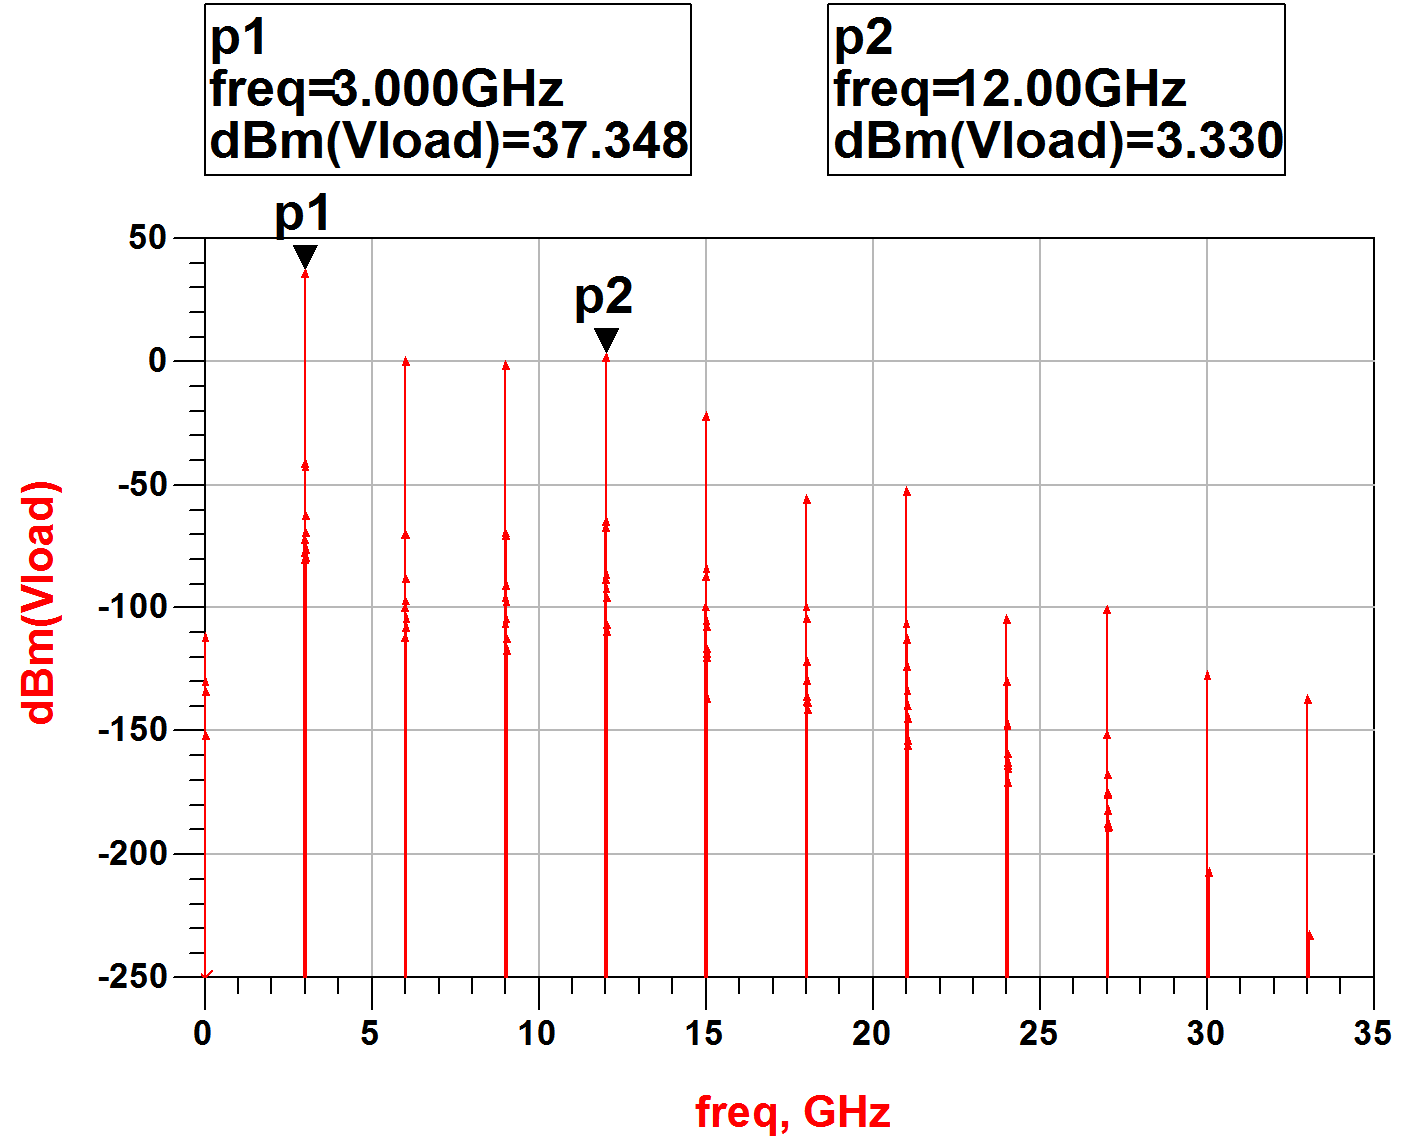
\includegraphics[width=5in,height=5in,keepaspectratio]{figures/amp_sim/IMD_twotone}\\
%  \caption{Simulated Two Tone IMD with 10 MHz Offset}
%  \label{fig:imd_double}
\end{figure}

\begin{figure}
  \centering
  % Requires \usepackage{graphicx}
  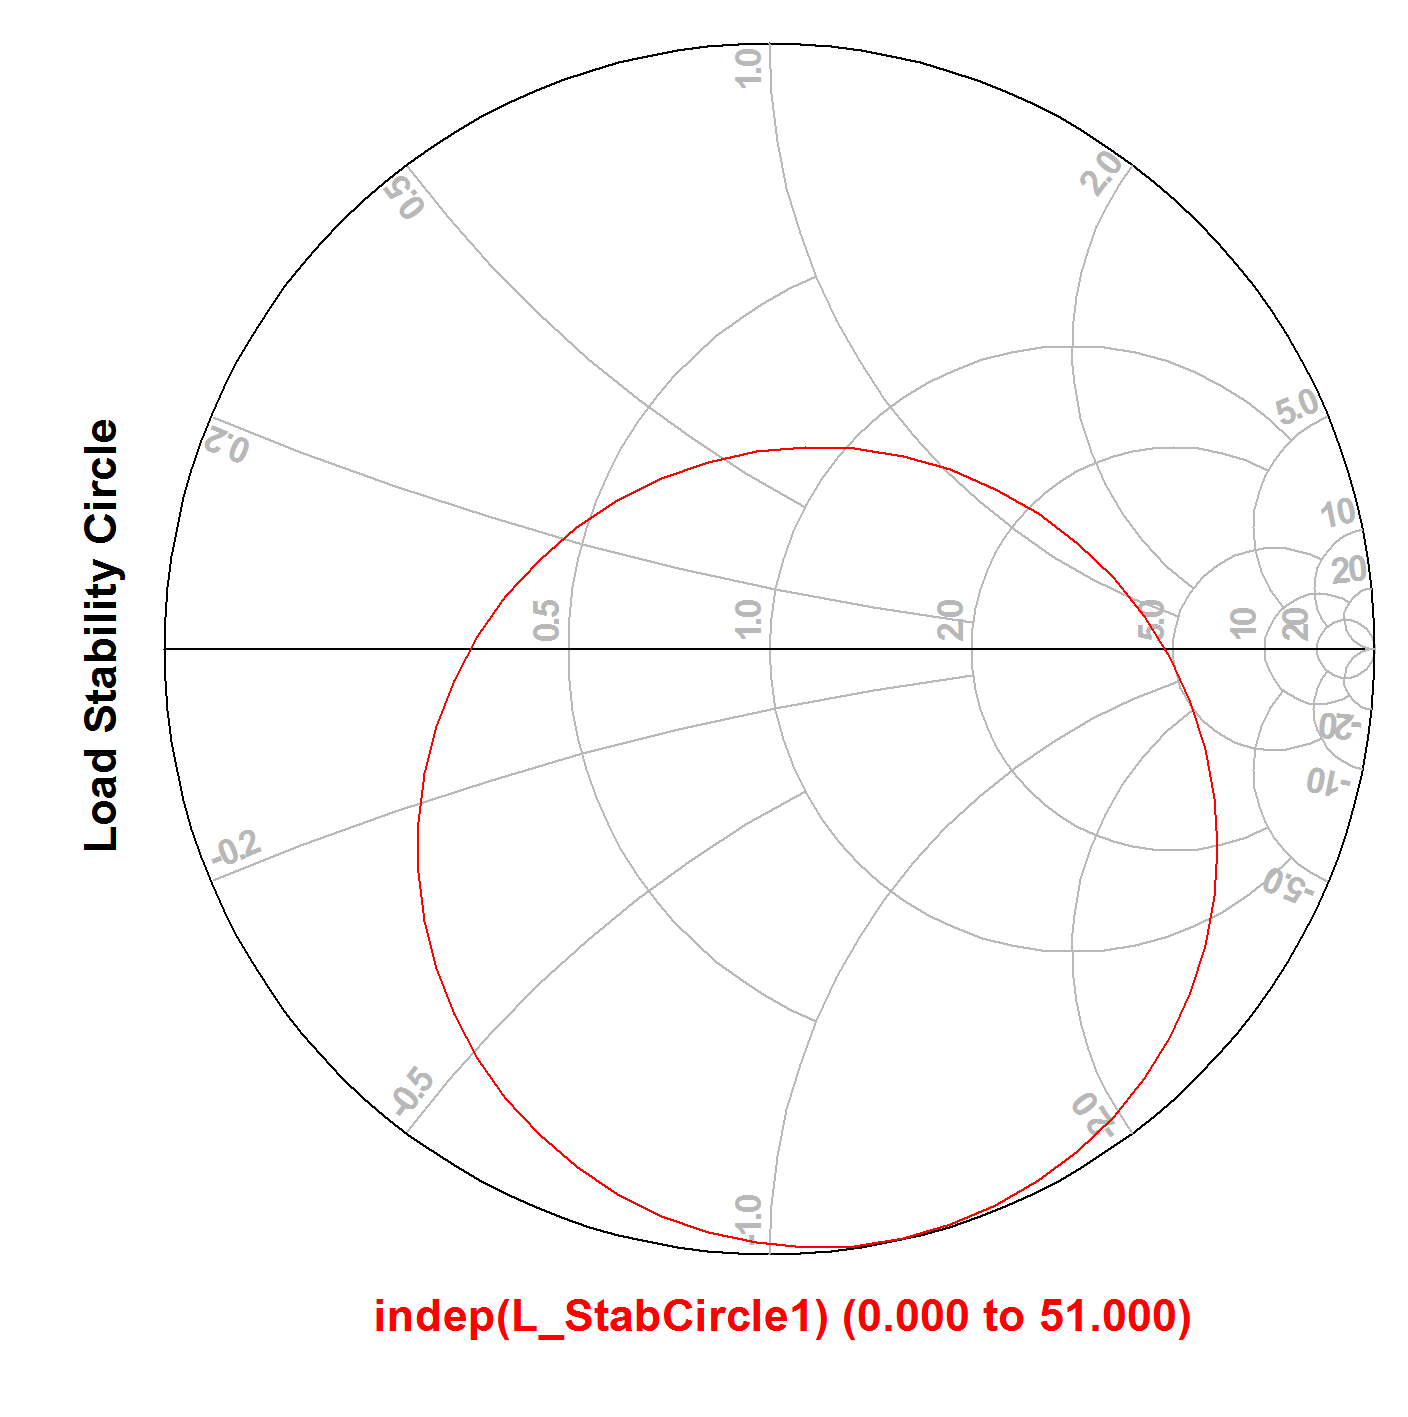
\includegraphics[width=4in,height=4in,keepaspectratio]{figures/amp_sim/load_stab_amp}\\
  \caption{Load Stability Circle of Amplifier. Stable Region Inside of Circle}
  \label{fig:amp_sim_load_stab}

  \vspace*{\floatsep}

  \centering
  % Requires \usepackage{graphicx}
  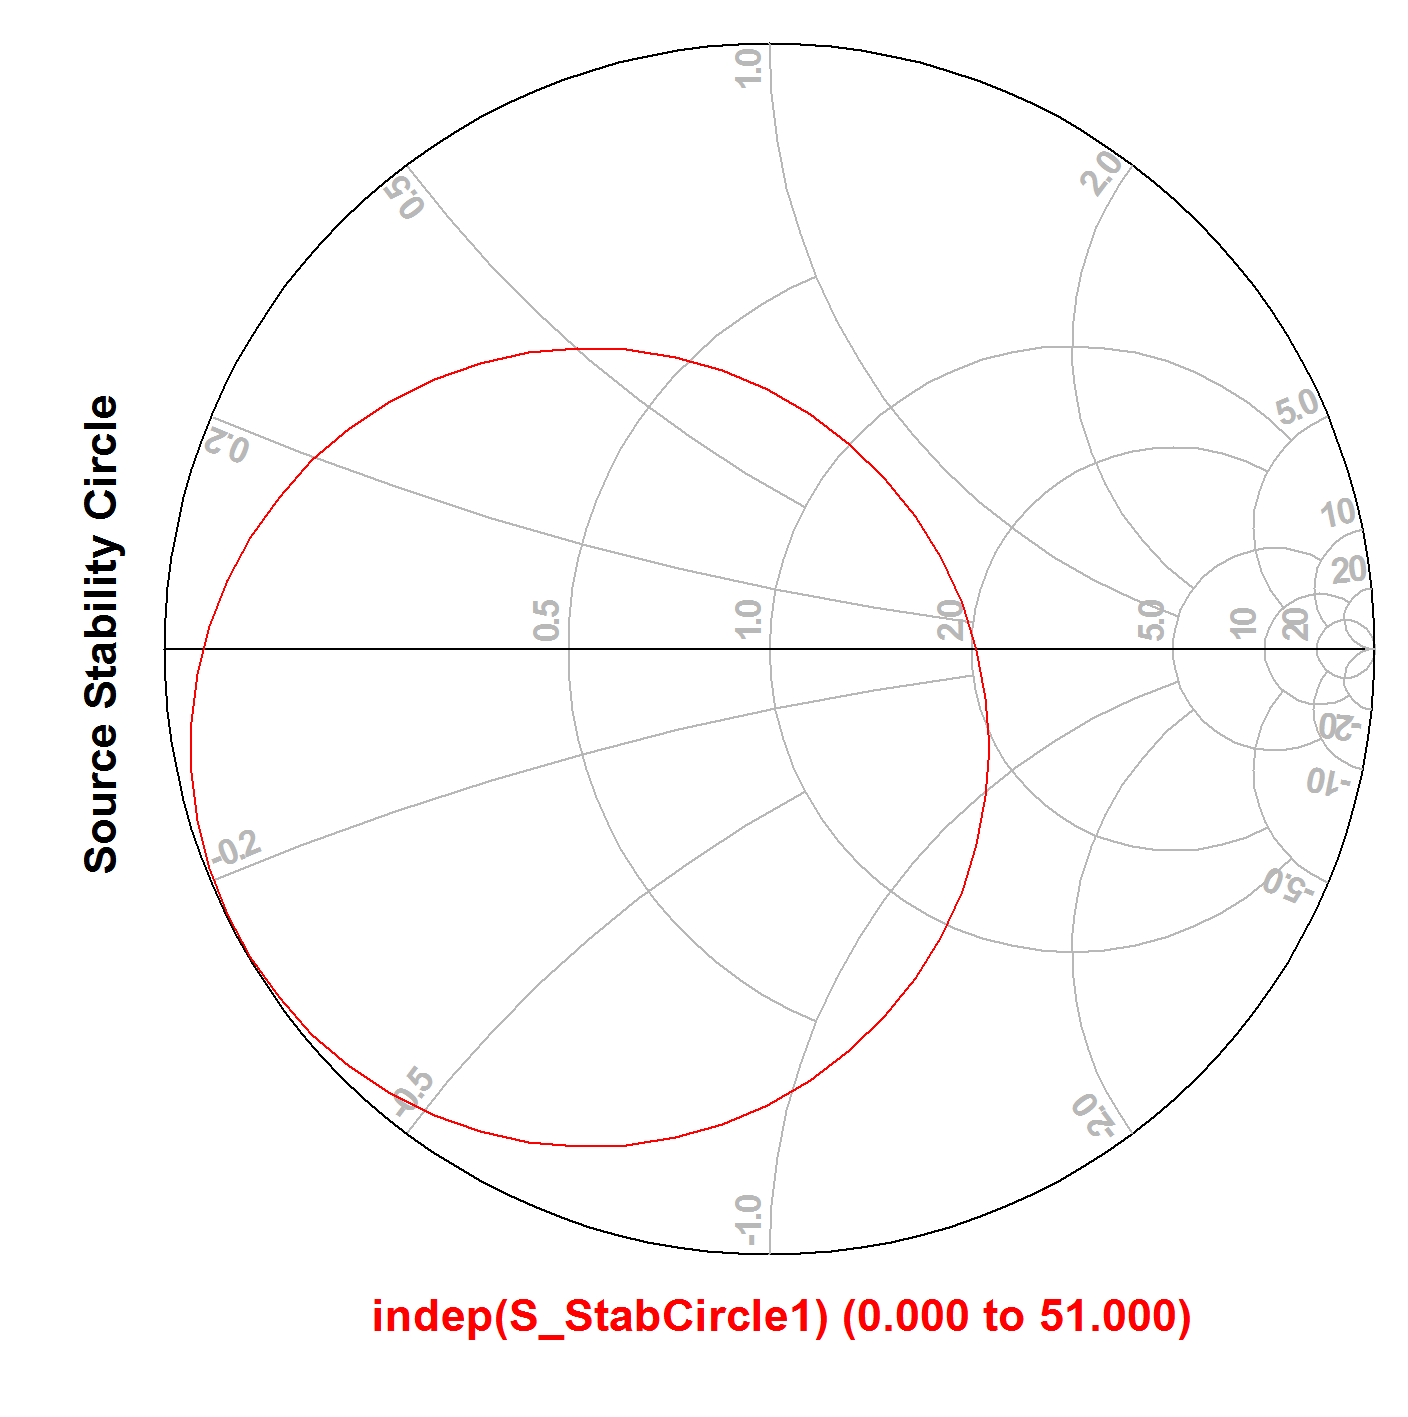
\includegraphics[width=4in,height=4in,keepaspectratio]{figures/amp_sim/source_stab_amp}\\
  \caption{Source Stability Circle of Amplifier. Stable Region Inside of Circle}
  \label{fig:amp_sim_source_stab}
\end{figure}


%VSWR plots
%How do get VSWR using harmonic balance? Fuck that shit got some dope ass plots
%
%Harmonic distortion plots
%
%Table of simulated amplifier measurements
%
%Board gerber files?

